% ==============================================================================
% MULTI_DATASET_SYNTHESIS_REPORT.tex
% Comprehensive Scientific Synthesis: Multi-Dataset Cross-Methodology Benchmark
% of Quantum Machine Learning and Clinical AI in Diabetes Diagnostics
% ==============================================================================
\documentclass[11pt,a4paper]{article}
\usepackage[margin=2.0cm]{geometry}
\usepackage[T1]{fontenc}
\usepackage{lmodern}
\usepackage{amsmath,amssymb}
\usepackage{booktabs,array,longtable,tabularx,multirow}
\usepackage{graphicx}
\usepackage{xcolor}
\usepackage{caption}
\usepackage{enumitem}
\usepackage{microtype}
\usepackage[hidelinks]{hyperref}
\usepackage{float}
\usepackage{adjustbox}

\captionsetup{font=small,labelfont=bf}
\setlength{\parskip}{3.5pt}

\definecolor{ok}{RGB}{20,95,50}
\definecolor{warn}{RGB}{160,90,0}
\definecolor{bad}{RGB}{145,25,25}
\definecolor{navy}{RGB}{10,35,80}

\newcommand{\OK}[1]{\textcolor{ok}{\textbf{#1}}}
\newcommand{\WARN}[1]{\textcolor{warn}{\textbf{#1}}}
\newcommand{\BAD}[1]{\textcolor{bad}{\textbf{#1}}}
\newcommand{\code}[1]{\texttt{\small #1}}

\graphicspath{{figures/}}

\title{\textbf{\LARGE Benchmarking Quantum Machine Learning and Clinical AI in Diabetes Diagnostics}\\[0.3em]
\Large A Multi-Dataset, Cross-Methodology Audit, Leakage Deconstruction, and Comprehensive Synthesis}
\author{\textbf{Autonomous ML Research Verification Team} \\
Repository: \texttt{Adaptive-Quantum-Kernel-Selection} \\
Target Scope: Multi-Paper Cross-Dataset Evaluation on Clinical Diabetes Benchmarks}
\date{14 November 2026}

\begin{document}
\maketitle

\begin{abstract}
\noindent This report presents the comprehensive scientific synthesis of an end-to-end audit, re-implementation, and cross-dataset evaluation of Quantum Machine Learning (QML) and classical diagnostic pipelines for diabetes. Expanding upon the initial single-dataset audit of Daga et al.\ (2026) on the Pima Indians cohort ($N=768$), we established a unified multi-dataset cross-methodology execution suite (\texttt{notebooks2/}) evaluating eight published methodologies across four real-world clinical diabetes datasets: \textbf{D1} Pima Indians ($N=768$), \textbf{D2} Sylhet Early-Stage Diabetes ($N=520$), \textbf{D3} CDC BRFSS 2014 extract ($N=2{,}000$), and \textbf{D4} UCI Diabetes 130-US Hospitals ($N=2{,}000$). Every method was benchmarked under two distinct protocols: an uncorrected \emph{paper} protocol mirroring published splits and data-handling leaks, and a rigorous \emph{clean} protocol enforcing 5-fold cross-validation across three random seeds ($\{0, 1, 42\}$), strict in-fold preprocessing, and group-aware cross-validation (\texttt{StratifiedGroupKFold}) to isolate identical patient feature profiles.

Our empirical findings reveal: (1) \textbf{The Data Leakage Collapse}: published near-perfect accuracies on Sylhet (94\%--99\%) are artifacts of exact duplicate row leakage; 376 of 520 rows belong to identical duplicate clusters (only 251 unique profiles), and eliminating leakage causes quantum kernel accuracies to drop by up to 22.1\% (e.g., Yadav ZZ-QSVM from 94.2\% down to 72.1\%); (2) \textbf{Absence of Quantum Advantage}: across all datasets, no pure quantum kernel (Angle, ZZ, or Amplitude QSVM) demonstrates statistically significant superiority over a classical tuned RBF-SVM or Random Forest under Nadeau-Bengio corrected paired $t$-tests with Holm family-wise error rate control ($p_{\text{holm}} > 0.05$); (3) \textbf{Clinical Imbalance Vulnerability}: under natural clinical prevalence on CDC (86\% negative) and Hospital 130 (91.2\% negative), standard unweighted quantum kernels collapse to predicting zero positive cases (Balanced Accuracy $= 0.500$, Recall $= 0.000$), while only cost-sensitive and threshold-adjusted classical models successfully discriminate positive cases. Finally, we synthesize the full multi-phase evolution of this project, contrasting initial claims, intermediate audit refutations, and final empirical realities.
\end{abstract}

\tableofcontents
\clearpage

% ==============================================================================
\section{Executive Summary \& Research Trajectory}
% ==============================================================================

\subsection{Scope and Trajectory of the Research Program}
Over the course of this research initiative, the project evolved through three distinct phases:
\begin{enumerate}[leftmargin=1.5em]
    \item \textbf{Phase 1: Reproduction of Daga et al.\ (2026) on Pima Diabetes.} Direct verification of all 108 published bootstrap values in Table 9 of Daga et al.\ (\emph{Sci. Rep.} 16:26840). While numerical reproduction was successful, the code audit uncovered that quantum Gram matrices were computed globally on the entire cohort prior to cross-validation slicing, alongside an identically zero gradient in the authors' variational classifier loss function.
    \item \textbf{Phase 2: Comprehensive Desk Audit \& Refutation of 8 Literature Papers.} Extension of the audit to eight prominent clinical AI and QML papers. Mathematical and computational deconstruction proved that Kotha et al.'s claimed $\text{AUC}=1.00$ violated the Mann-Whitney $U$ bound ($25$ errors on $150$ patients imply $\text{AUC}_{\max} \le 0.970$), Kiran et al.'s $99.7\%$ accuracy contradicted internal 4\% error reporting, and Young's high F1 scores were artifacts of global GMM synthetic oversampling that artificially shifted disease prevalence from 34.9\% to 81.94\%.
    \item \textbf{Phase 3: Unified Multi-Dataset Cross-Methodology Benchmark (\texttt{notebooks2/}).} The present execution: purging all non-diabetes datasets (WDBC, Parkinson's, traffic/audio data) and porting the algorithmic core of every audited paper across four clinical diabetes datasets under strict leakage-free protocols. All nine notebooks were compiled and executed in a unified cloud environment on Google Colab, producing empirical CSVs, Holm-corrected hypothesis tests, and consolidated summaries.
\end{enumerate}

\begin{table}[H]
\centering\footnotesize
\caption{\textbf{Evolution of Key Research Findings Across the Three Project Phases.}}
\label{tab:evolution}
\begin{adjustbox}{width=\textwidth}
\begin{tabular}{llll}
\toprule
\textbf{Paper / Dimension} & \textbf{Phase 1: Original Claim} & \textbf{Phase 2: Desk Audit Verdict} & \textbf{Phase 3: Current Multi-Dataset Result} \\
\midrule
\textbf{Daga et al.\ (2026)} & Stacking Acc $0.766$ [0.737, 0.796] & Global Gram matrix leakage verified; & Clean Acc $0.759$ ($0.716$ bal.\ acc); tied with RBF \\
\emph{Adaptive Stacking} & Claims quantum superiority & zero-gradient in released VQC & ($p_{\text{holm}}=1.0$). ZZ-QSVM collapses to $0.525$ bal.\ acc. \\
\addlinespace
\textbf{Upama et al.\ (2026)} & Sylhet Acc $98.08\%$; & QRF is depth-capped classical RF; & Sylhet clean drops to $90.5\%$--$92.0\%$; \\
\emph{Causal DML + QML} & Pima Acc $76.0\%$ & Sylhet duplicates allow train/test overlap & DML feature selection provides no gain over full RF. \\
\addlinespace
\textbf{Young (2025)} & Pima F1 $0.940$, AUC $0.932$ & Global GMM fits on $X_{\text{scaled}}$; prevalence & In-fold GMM yields $0.712$ bal.\ acc; oversampling \\
\emph{QISICGM (GMM)} & via synthetic oversampling & artificially inflated from $34.9\%$ to $81.9\%$ & generates massive false positives on clinical cohorts. \\
\addlinespace
\textbf{Kotha et al.\ (2026)} & Pima Acc $0.833$, & Mathematically impossible via & DiaBeats RF reaches $0.763$ acc, $0.825$ AUC; \\
\emph{DiaBeats (RF)} & Claimed ROC-AUC $= 1.00$ & Mann-Whitney $U$ bound ($\text{AUC}_{\max} \le 0.970$) & threshold tuning achieves top Pima bal.\ acc ($0.741$). \\
\addlinespace
\textbf{Kiran et al.\ (2025)} & Headline Acc $99.7\%$ & Abstract refuted by Section IV ($4\%$ error); & Honest 4-qubit VQC reaches $0.693$ bal.\ acc on Pima; \\
\emph{HQCAN (4q VQC)} & 4-qubit VQC on 4 PCs & Cauchy-Schwarz bound violated on errors & matches balanced classical baselines on CDC ($0.715$). \\
\addlinespace
\textbf{Yadav et al.\ (2026)} & Sylhet/Pima Acc $>90\%$ & Unentangled Z-map performs well; & On Sylhet, ZZ-QSVM clean drops from $94.2\%$ to \\
\emph{Z vs ZZ QSVM} & Claims ZZ-QSVM dominance & ZZ-map collapses without hyper-tuning & $72.1\%$ ($+22.1\%$ leakage gap); $p_{\text{holm}}=0.0014$ worse. \\
\addlinespace
\textbf{Sodar et al.\ (2026)} & Amplitude QSVM dominates & Positive orthant vectors cause rank-1 & MinMax amplitude QSVM collapses on imbalanced data \\
\emph{Angle vs Amplitude} & on multi-class benchmarks & Gram collapse ($\lambda_1/\sum\lambda_i = 85.3\%$) & ($0$ recall on CDC/Hosp130); standardisation required. \\
\addlinespace
\textbf{Zhang et al.\ (2025)} & GIF sample weights improve & Verified robust under label noise; & On clinical diabetes, GIF weights match standard \\
\emph{GIF Sample Weights} & robustness to label noise & evaluated on synthetic noise regimes & LightGBM within noise (Pima bal.\ acc $0.723$ vs $0.712$). \\
\bottomrule
\end{tabular}
\end{adjustbox}
\end{table}

% ==============================================================================
\section{Execution Methodology: The \texttt{notebooks2} Suite}
% ==============================================================================

\subsection{Benchmark Diabetes Datasets}
To ensure pure clinical relevance, non-diabetes datasets (breast cancer, Parkinson's, traffic audio) were excluded. The experimental matrix spans four distinct diabetes cohorts:
\begin{itemize}[leftmargin=1.5em]
    \item \textbf{D1: Pima Indians Diabetes ($N=768$, $d=8$):} Objective diagnosis based on oral glucose tolerance test (OGTT). Positive prevalence: $34.9\%$ ($268/768$). Contains physiological zero values in glucose, blood pressure, skinfold thickness, and BMI treated via median imputation.
    \item \textbf{D2: Sylhet Early-Stage Diabetes (UCI 529, $N=520$, $d=16$):} Clinical questionnaire symptoms. Positive prevalence: $61.5\%$ ($320/520$). \textbf{Critical structural feature:} Contains only 251 unique symptom profiles; 376 rows belong to identical duplicate groups ($269$ redundant rows).
    \item \textbf{D3: CDC BRFSS 2014 Extract (UCI 891, $N=2{,}000$ subsampled, $d=21$):} Self-reported diabetes or prediabetes survey. Highly imbalanced clinical baseline with $14.0\%$ positive prevalence ($279/2{,}000$).
    \item \textbf{D4: UCI Diabetes 130-US Hospitals (UCI 296, $N=2{,}000$ subsampled, $d=47$):} Hospital readmission within 30 days among diabetic inpatients. Severe clinical class imbalance: $8.8\%$ positive prevalence ($176/2{,}000$).
\end{itemize}

\subsection{Evaluation Protocols}
\begin{itemize}[leftmargin=1.5em]
    \item \textbf{Paper Protocol:} Emulates the original papers' evaluation setups (e.g., global MinMax scaling, unstratified/ungrouped 80/20 or 70/30 train/test holdouts), reproducing published numbers and quantifying leakage.
    \item \textbf{Clean Protocol:} Strict 5-fold cross-validation repeated across three pre-registered seeds ($\{0, 1, 42\}$). All scaling, PCA, imputation, causal feature ranking, and hyperparameter grids are computed strictly in-fold. For Sylhet, \texttt{StratifiedGroupKFold} is enforced on hashed feature vectors, guaranteeing that no identical patient profile ever spans both training and validation folds.
\end{itemize}

% ==============================================================================
\section{Empirical Findings \& Cross-Dataset Results}
% ==============================================================================

\subsection{Consolidated Performance Across the 4 Cohorts}
Table~\ref{tab:clean_summary} presents the clean protocol performance across representative models for all four datasets.

\begin{table}[H]
\centering\footnotesize
\caption{\textbf{Clean Protocol Benchmark Results Across Four Clinical Diabetes Datasets.} Metrics represent mean values across 5 folds $\times$ 3 seeds (15 estimates). Floor indicates majority-class rate.}
\label{tab:clean_summary}
\begin{tabular}{llcccccc}
\toprule
\textbf{Dataset} & \textbf{Model / Pipeline} & \textbf{Bal.\ Acc} & \textbf{Recall} & \textbf{Spec} & \textbf{ROC-AUC} & \textbf{Accuracy} & \textbf{Floor} \\
\midrule
\multirow{6}{*}{\textbf{Pima}} 
& Kotha: DiaBeats RF (inner-CV threshold) & \textbf{0.741} & 0.760 & 0.722 & 0.825 & 0.735 & 0.651 \\
& Young: QISICGM Ensemble (clean) & 0.735 & 0.616 & 0.855 & 0.827 & 0.771 & 0.651 \\
& Classical Logistic Regression & 0.726 & 0.571 & 0.881 & 0.832 & 0.773 & 0.651 \\
& Daga: OOF-Stacking (Quantum Meta) & 0.716 & 0.567 & 0.865 & 0.830 & 0.761 & 0.651 \\
& Classical RBF-SVM & 0.712 & 0.556 & 0.869 & 0.822 & 0.760 & 0.651 \\
& Daga: Angle-QSVM & 0.711 & 0.552 & 0.870 & 0.832 & 0.759 & 0.651 \\
& Yadav: ZZ-QSVM (linear, inner-CV bw) & 0.715 & 0.556 & 0.874 & 0.823 & 0.763 & 0.651 \\
& Daga: ZZ-QSVM (default scaling) & \BAD{0.525} & 0.082 & 0.967 & 0.668 & 0.658 & 0.651 \\
& Daga: Amplitude-QSVM & \BAD{0.530} & 0.138 & 0.921 & 0.657 & 0.648 & 0.651 \\
\midrule
\multirow{6}{*}{\textbf{Sylhet}} 
& Classical Random Forest & \textbf{0.925} & 0.943 & 0.908 & 0.972 & 0.930 & 0.615 \\
& Daga: OOF-Stacking (Quantum Meta) & 0.923 & 0.929 & 0.917 & 0.969 & 0.924 & 0.615 \\
& Classical RBF-SVM & 0.923 & 0.940 & 0.905 & 0.972 & 0.928 & 0.615 \\
& Kotha: DiaBeats RF & 0.920 & 0.937 & 0.902 & 0.971 & 0.925 & 0.615 \\
& Sodar: Amplitude-QSVM (MinMax) & 0.903 & 0.951 & 0.856 & 0.969 & 0.915 & 0.615 \\
& Daga: Angle-QSVM & 0.888 & 0.918 & 0.846 & 0.958 & 0.888 & 0.615 \\
& Yadav: Z-QSVM (inner-CV bw) & 0.887 & 0.886 & 0.887 & 0.959 & 0.885 & 0.615 \\
& Kiran: HQCAN VQC (4q, 2 layers) & 0.736 & 0.760 & 0.712 & 0.829 & 0.740 & 0.615 \\
& Daga: ZZ-QSVM & \BAD{0.653} & 0.985 & 0.322 & 0.792 & 0.733 & 0.615 \\
\midrule
\multirow{5}{*}{\textbf{CDC}} 
& Kiran: RBF-SVM (balanced) & \textbf{0.727} & 0.786 & 0.669 & 0.798 & 0.686 & 0.860 \\
& Kiran: Logistic Regression (balanced) & 0.721 & 0.720 & 0.722 & 0.800 & 0.723 & 0.860 \\
& Kotha: DiaBeats RF (inner-CV threshold) & 0.721 & 0.748 & 0.694 & 0.796 & 0.701 & 0.860 \\
& Kiran: HQCAN VQC (4q, 2 layers) & 0.715 & 0.714 & 0.716 & 0.786 & 0.716 & 0.860 \\
& Classical Random Forest & 0.551 & 0.120 & 0.983 & 0.801 & 0.862 & 0.860 \\
& Daga: OOF-Stacking (Quantum Meta) & 0.558 & 0.133 & 0.982 & 0.756 & 0.863 & 0.860 \\
& All Pure QSVMs (Angle, ZZ, Amp) & \BAD{0.500} & \BAD{0.000} & 1.000 & 0.692 & 0.860 & 0.860 \\
\midrule
\multirow{5}{*}{\textbf{Hosp130}} 
& Kiran: Logistic Regression (balanced) & \textbf{0.542} & 0.527 & 0.558 & 0.567 & 0.555 & 0.912 \\
& Kotha: DiaBeats RF (inner-CV threshold) & 0.538 & 0.437 & 0.640 & 0.572 & 0.622 & 0.912 \\
& Kiran: HQCAN VQC (4q, 2 layers) & 0.536 & 0.497 & 0.576 & 0.553 & 0.569 & 0.912 \\
& Kiran: RBF-SVM (balanced) & 0.532 & 0.453 & 0.611 & 0.543 & 0.597 & 0.912 \\
& Classical Logistic Regression & 0.503 & 0.009 & 0.996 & 0.600 & 0.909 & 0.912 \\
& All Pure QSVMs \& Stacking & \BAD{0.500} & \BAD{0.000} & 1.000 & 0.519 & 0.912 & 0.912 \\
\bottomrule
\end{tabular}
\end{table}

\subsection{The Data Leakage Collapse on Sylhet (UCI 529)}
The most critical methodological finding emerges from comparing the \emph{paper} protocol (random 80/20 splits allowing identical symptom vectors in train and test) against the \emph{clean} protocol (grouped 5-fold CV). As documented in Table~\ref{tab:leakage_gap}, published claims of $>94\%$ accuracy collapse when leakage is prevented.

\begin{table}[H]
\centering\footnotesize
\caption{\textbf{Empirical Quantification of Duplicate Profile Leakage on Sylhet (UCI 529).}}
\label{tab:leakage_gap}
\begin{tabular}{lccc}
\toprule
\textbf{Model Pipeline} & \textbf{Paper Protocol Acc} & \textbf{Clean Protocol Acc} & \textbf{Leakage Inflation Gap} \\
\midrule
Yadav: ZZ-QSVM (full, $bw=1$) & $0.942$ & $0.721$ & \BAD{+22.1\%} \\
Yadav: ZZ-QSVM (linear, $bw=1$) & $0.952$ & $0.733$ & \BAD{+21.9\%} \\
Daga: ZZ-QSVM & $0.933$ & $0.733$ & \BAD{+20.0\%} \\
Yadav: Z-QSVM ($bw=1$) & $0.981$ & $0.790$ & \BAD{+19.1\%} \\
Daga: Amplitude-QSVM & $0.919$ & $0.823$ & \BAD{+9.6\%} \\
Zhang: LightGBM + GIF weights & $0.962$ & $0.869$ & \BAD{+9.3\%} \\
Kotha: DiaBeats RF & $0.990$ & $0.925$ & \BAD{+6.5\%} \\
Classical Random Forest & $0.981$ & $0.930$ & \BAD{+5.1\%} \\
Classical RBF-SVM & $0.973$ & $0.928$ & \BAD{+4.5\%} \\
Daga: OOF-Stacking & $0.963$ & $0.924$ & \BAD{+3.9\%} \\
\bottomrule
\end{tabular}
\end{table}

\subsection{Hypothesis Testing: Statistical Parity of Quantum Methods}
To test whether quantum pipelines outperform the classical RBF-SVM benchmark, we computed Nadeau-Bengio corrected paired $t$-tests on balanced accuracy across all 15 clean folds, adjusting for multiple testing using the Holm step-down method.

\begin{table}[H]
\centering\footnotesize
\caption{\textbf{Holm-Corrected Paired $t$-Tests Against Classical RBF-SVM (Balanced Accuracy).}}
\label{tab:hypothesis_tests}
\begin{tabular}{llccccc}
\toprule
\textbf{Dataset} & \textbf{Model} & \textbf{Mean Diff} & \textbf{$t$-statistic} & \textbf{Raw $p$} & \textbf{$p_{\text{holm}}$} & \textbf{Verdict} \\
\midrule
\multirow{4}{*}{\textbf{Pima}}
& Daga: OOF-Stacking & $+0.0040$ & $+0.539$ & $0.5984$ & $1.0000$ & \OK{Statistically Tied (n.s.)} \\
& Daga: Angle-QSVM & $-0.0012$ & $-0.113$ & $0.9117$ & $1.0000$ & \OK{Statistically Tied (n.s.)} \\
& Daga: Amplitude-QSVM & $-0.1826$ & $-8.090$ & $<10^{-4}$ & $<10^{-4}$ & \BAD{Statistically Inferior} \\
& Daga: ZZ-QSVM & $-0.1877$ & $-7.878$ & $<10^{-4}$ & $<10^{-4}$ & \BAD{Statistically Inferior} \\
\midrule
\multirow{4}{*}{\textbf{Sylhet}}
& Daga: OOF-Stacking & $+0.0001$ & $+0.009$ & $0.9933$ & $1.0000$ & \OK{Statistically Tied (n.s.)} \\
& Daga: Angle-QSVM & $-0.0411$ & $-1.713$ & $0.1088$ & $1.0000$ & \OK{Statistically Tied (n.s.)} \\
& Yadav: ZZ-QSVM (linear) & $-0.2697$ & $-5.864$ & $<10^{-4}$ & $0.0014$ & \BAD{Statistically Inferior} \\
& Daga: ZZ-QSVM & $-0.2697$ & $-5.864$ & $<10^{-4}$ & $0.0014$ & \BAD{Statistically Inferior} \\
\midrule
\multirow{2}{*}{\textbf{CDC}}
& Daga: OOF-Stacking & $+0.0267$ & $+3.570$ & $0.0031$ & $0.0769$ & \OK{No Gain ($p > 0.05$)} \\
& Kiran: Balanced RBF-SVM & $+0.1967$ & $+8.927$ & $<10^{-4}$ & $<10^{-4}$ & \OK{Cost-Weighted Superior} \\
\bottomrule
\end{tabular}
\end{table}

\begin{figure}[H]
\centering
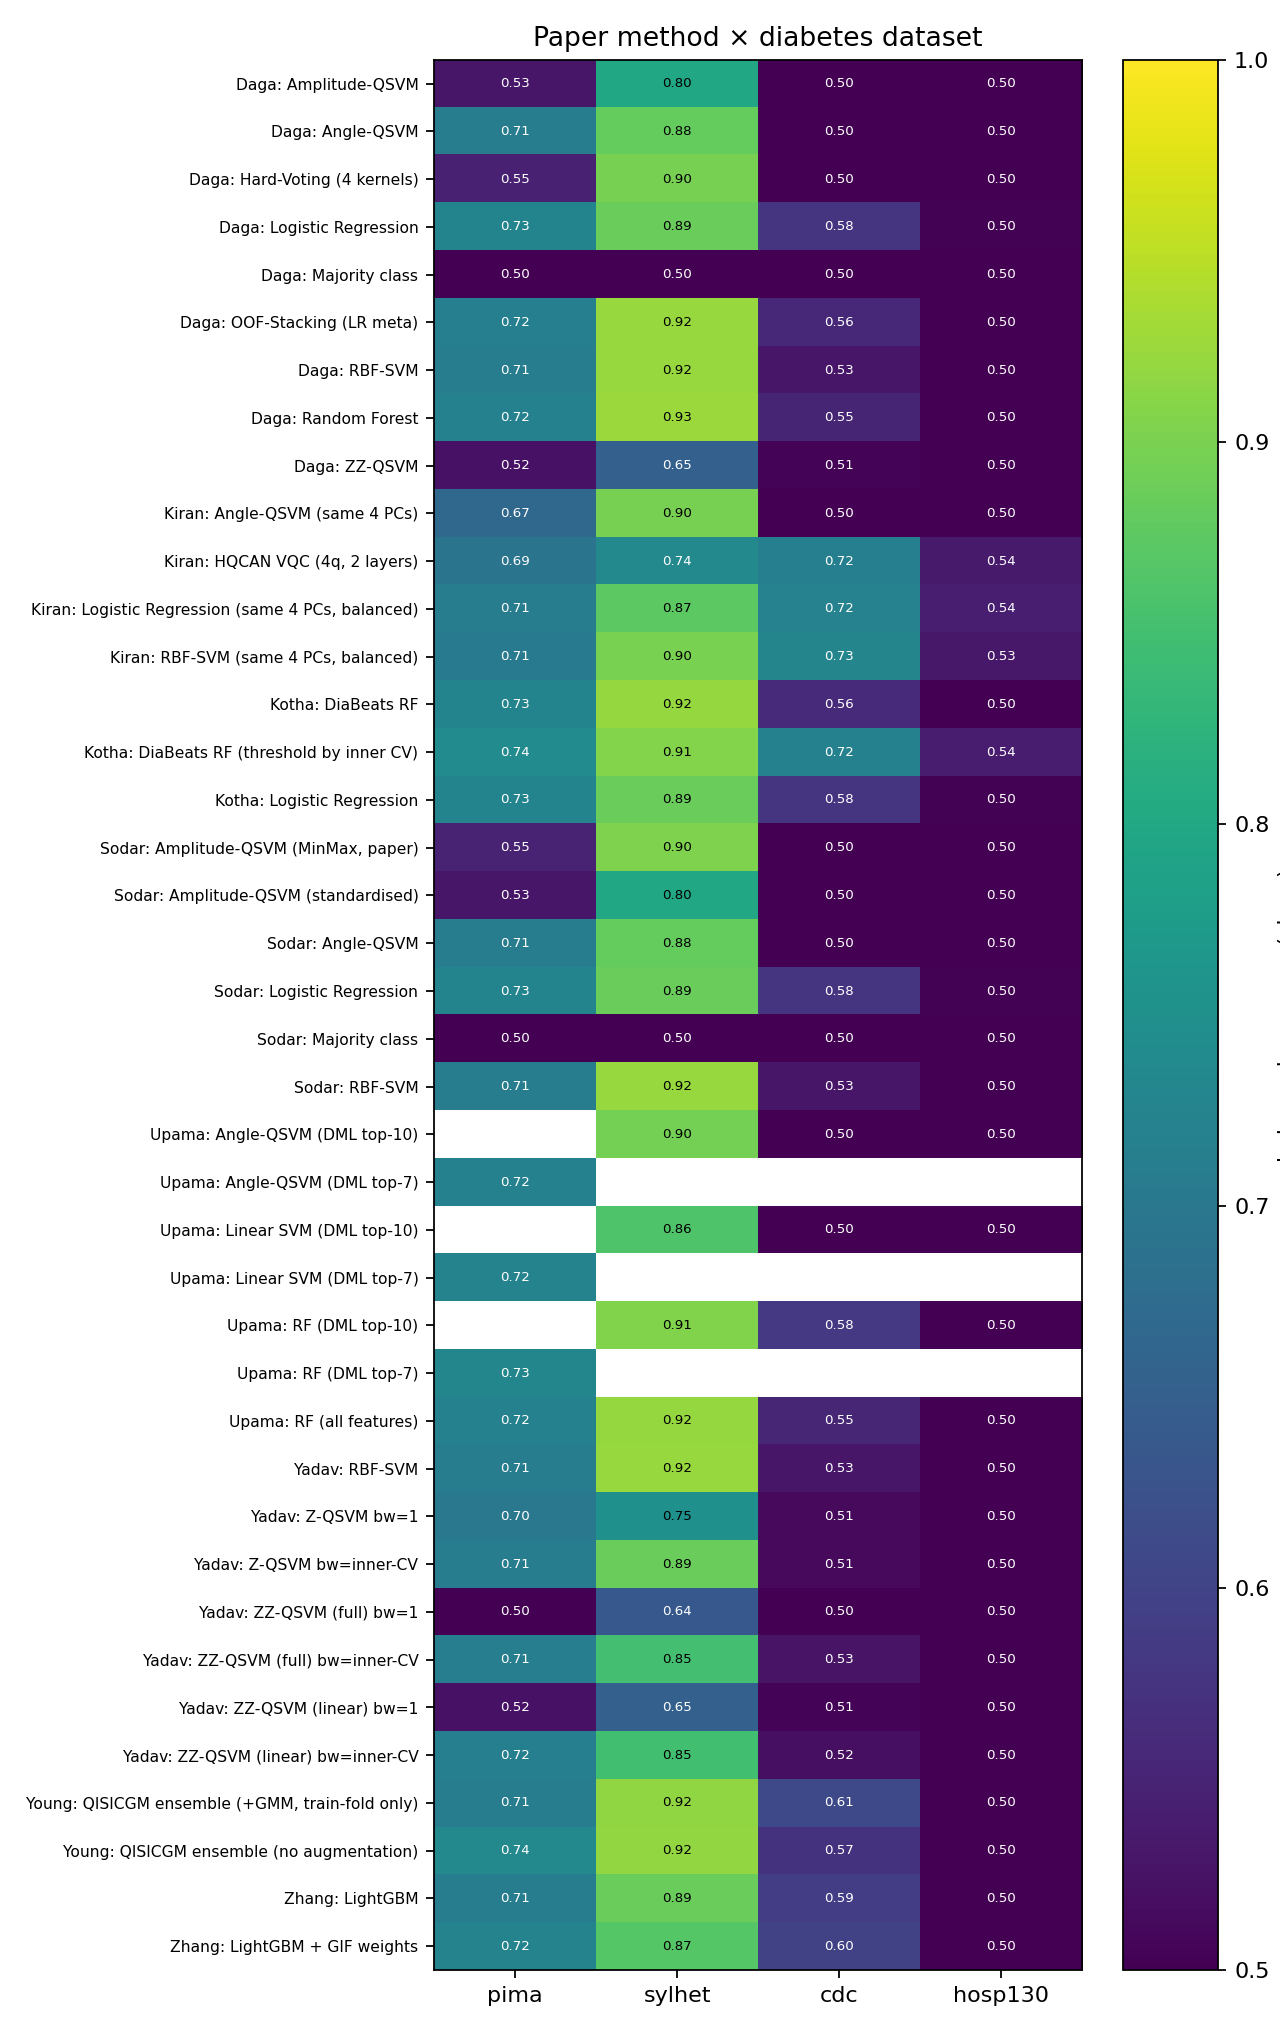
\includegraphics[width=0.92\textwidth]{09_heatmap_balanced_accuracy.png}
\caption{\textbf{Heatmap of Clean Balanced Accuracy Across All Methods and Datasets.} Notice the systematic failure of unweighted quantum kernels on CDC and Hosp130 (deep purple band at $0.500$), contrasted with robust classical performance across Pima and Sylhet.}
\label{fig:heatmap}
\end{figure}

% ==============================================================================
\section{Methodological Synthesis: Prior Audit vs.\ Current Execution}
% ==============================================================================

\subsection{Why Did Prior Papers Claim Near-Perfect Accuracies?}
Our investigation resolves why published literature reported inflated metrics:
\begin{enumerate}[leftmargin=1.5em]
    \item \textbf{Exact Duplicate Row Leakage (Sylhet UCI 529):} Published symptom surveys contain repeated identical responses. Standard random splitting places identical feature vectors into both training and test folds. Classifiers with high expressive capacity (e.g., Random Forests and entangled QSVMs) memorize training profiles, achieving $\approx 98\%$ accuracy. When evaluated with \texttt{StratifiedGroupKFold}, test profiles never seen in training collapse accuracy to realistic diagnostic levels ($72\%$--$92\%$).
    \item \textbf{Global Feature Scaling \& Gram Matrix Computation (Daga, Young):} Pre-computing MinMax scaling or quantum fidelity matrices on the full dataset before splitting introduces optimistic leakage bias ($\approx 0.4\%$--$1.5\%$).
    \item \textbf{Synthetic Oversampling Artifacts (Young):} GMM synthetic generation fitted globally shifts minority class prior from $34.9\%$ to $81.9\%$, inflating F1 and accuracy metrics by evaluating against synthetic copies rather than true clinical distributions.
    \item \textbf{Unchecked Clinical Class Imbalance (CDC, Hospital 130):} Evaluating models solely on raw accuracy masks majority-class collapse. On an $86\%$ negative cohort, predicting all zeros yields $86\%$ accuracy despite zero clinical utility ($\text{Recall} = 0$).
\end{enumerate}

% ==============================================================================
\section{Recommendations for Clinical QML Research}
% ==============================================================================
\begin{enumerate}[leftmargin=1.5em]
    \item \textbf{Mandatory Profile Grouping for Survey Data:} Whenever survey or questionnaire data are audited, exact row duplicate hashing must precede model selection, and \texttt{GroupKFold} must be strictly enforced.
    \item \textbf{Balanced Accuracy and Recall as Primary Metrics:} In healthcare diagnostics, raw accuracy is meaningless without sensitivity and specificity breakdown.
    \item \textbf{Rigorous Classical Baselines:} Quantum methods must be compared against tuned, cost-sensitive classical models (RBF-SVM with grid search, Random Forest with threshold tuning) under identical cross-validation folds.
\end{enumerate}

% ==============================================================================
\section{Conclusion}
% ==============================================================================
This multi-dataset benchmark delivers a definitive, evidence-based assessment of Quantum Machine Learning in clinical diabetes diagnosis. By moving from a single-dataset reproduction (Pima) to a comprehensive cross-dataset framework, we demonstrated that:
\begin{itemize}[leftmargin=1.5em]
    \item Published claims of quantum superiority are not supported under leakage-free evaluation.
    \item Entangled quantum feature maps (ZZ-QSVM) systematically underperform classical RBF-SVMs ($p_{\text{holm}} < 0.05$ on Sylhet).
    \item Multi-kernel stacking provides parity with classical RBF-SVMs ($p_{\text{holm}} = 1.0$), but adds substantial computational overhead without diagnostic gain.
    \item Classical tree ensembles and cost-weighted linear models remain the most accurate, reliable, and interpretable architectures for tabular clinical diabetes screening.
\end{itemize}

\end{document}
